\chapter{Implémentation} \label{intro}
%------------------------------------------
\section{Introduction}
    Dans ce qui précède nous avons présenté  la recherche basée sur la similarité et l'ontologie. Dans ce chapitre Nous allons expliquer  comment nous avons exploité les connaissances cultivées durant la phase de la documentation afin d'implémenter un système qui permet d'effectuer une recherche sémantique dans le but de découvrir les services Cloud similaires aux besoins de l'utilisateur.\\
    Dans ce chapitre nous allons présenter les principaux outils du développement de notre application. Ensuite, nous allons expliquer la conception de notre système. Finalement, nous présenterons la partie réalisation et tests.\\

\section{Outils de développement}
    Tout au long de la phase de l'implémentation nous avons utilisé plusieurs outils qui nous ont énormément aidés à réaliser notre application:
    \subsection{Environnement de développement et éditeurs}
        \begin{itemize}
            \item[\quad $\bullet$] Eclipse: C'est un environnement de développement open source parmi les environnements les  plus utilisé dans le monde pour le développement des produits logiciel sous plusieurs langages.
            \item[\quad $\bullet$] Protégé: C'est un éditeur d'ontologies open source. Il a été développé en java par l'Université de Stanford pour des raisons de recherche dans le domaine du web sémantique.
            \item[\quad $\bullet$] Produit de la firme Microsoft, WinEdit est un éditeur de texte. Il est très utilisé pour la rédaction des documents en LaTex
        \end{itemize}
    \subsection{Langages de programmation}
        \begin{itemize}
            \item[\quad $\bullet$] Java version 8: C'est un langage de programmation orienté objet développée par SunMicrosystems. Sa portabilité lui vaut le titre d'un des langages les plus utilisés au monde.
            \item[\quad $\bullet$] OWL: Langage de description d'ontologie. On l'a bien défini au premier chapitre.
            \item[\quad $\bullet$] LaTex: C'est un système de composition de haute qualité, il inclut des fonctionnalités conçues pour la production de la documentation technique et scientifique
            \item[\quad $\bullet$] UML: C'est un langage de modélisation et de conception basé sur les pictogrammes
        \end{itemize}
    \subsection{Autres outils}
        \begin{itemize}
            \item[\quad $\bullet$] Git: C'est un logiciel de gestion de versions décentralisé open source. Il permet à l'utilisateur de créer plusieurs versions de son travail pour éviter les pertes de documents. Il facilite le travail en équipe sur le même projet.
            \item[\quad $\bullet$] GitHub : c'est un outil qui joue le rôle  d'un support de stockage distant des différentes versions d'un projet.
            \item[\quad $\bullet$]PowerAMC Designer: C'est un logiciel de modélisation des diagramme UML.
        \end{itemize}

\section{Conception}
    La conception est une étape clé dans le cycle de vie de chaque produit logiciel. Elle permet de bien définir le produit, de le modéliser et mettre en relief ses différentes fonctionnalités. Pour réaliser la conception de notre système,nous avons utilisé le langage UML.\\
        \subsection{Diagramme des cas d'utilisation}
            Les cas d'utilisations décrivent les fonctionnalités fournies par le système à un acteur [Revuz 2014b]. Ils sont utilisés généralement par les clients, les concepteurs, les concepteurs et les testeurs.\\
            Dans notre cas l'utilisateur va saisir une requête dans le but qu'elle soit traité par le système. Mais pour que le traitement soit bien exécuté le système doit extraire les données à partir de l'ontologie.
            \begin{figure}[H]
                    \centering
                    % Requires \usepackage{graphicx}
                    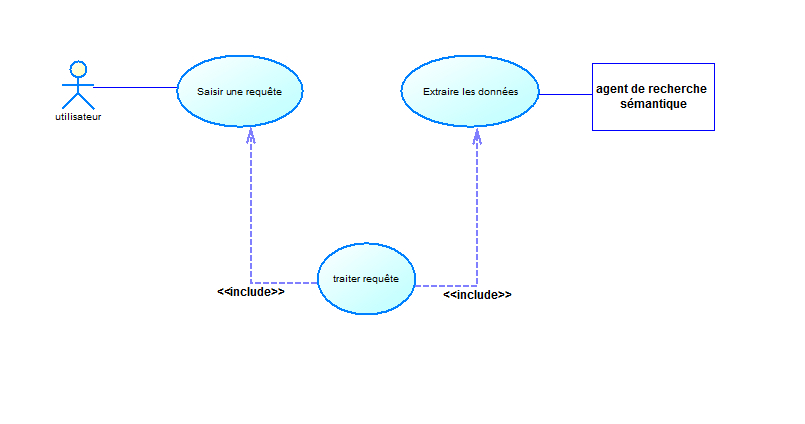
\includegraphics[width=20cm]{cas_utilisation}\\
                    \caption{diagramme des cas d'utilisation}\label{diagramme des cas d'utilisation}
            \end{figure}
        \subsection{Diagramme de séquences de point de vue système}
        Afin de décrire le scénario global de l'application nous avons proposé de construire le diagramme de séquences de point de vue système.\\
        Lorsque l'utilisateur saisit une requête , le système va procéder à son analyse. Deux cas se présentent:\\
        Dans le premier cas la requête contient une erreur de saisie. Donc le système va alors afficher un message d'erreur.\\
        Dans le deuxième  cas la requête est considéré comme valide donc le système procède au traitement nécessaire et retourne le résultat final à l'utilisateur.\\
        \begin{figure}[H]
                    \centering
                    % Requires \usepackage{graphicx}
                    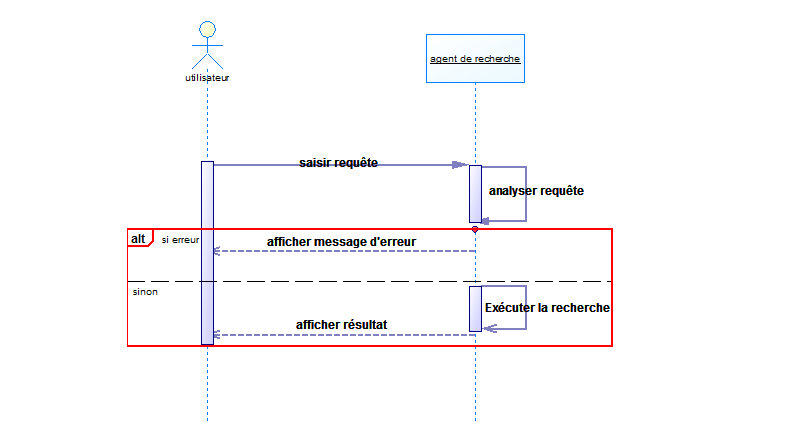
\includegraphics[width=20cm]{diagramme_sequence_system}\\
                    \caption{diagramme de sequences de point de vue systèm}\label{diagramme sequence system}
        \end{figure}
        \subsection{Diagramme de séquences détaillé}
        Suite à la déscription du  scénario général de l'application à travers le diagramme des séquences de point de vue système, on va maintenant décrire le fonctionnement et les interactions entre les différentes entités à l'aide d'un diagramme de séquences détaillé.\\
            \begin{figure}[H]
                    \centering
                    % Requires \usepackage{graphicx}
                    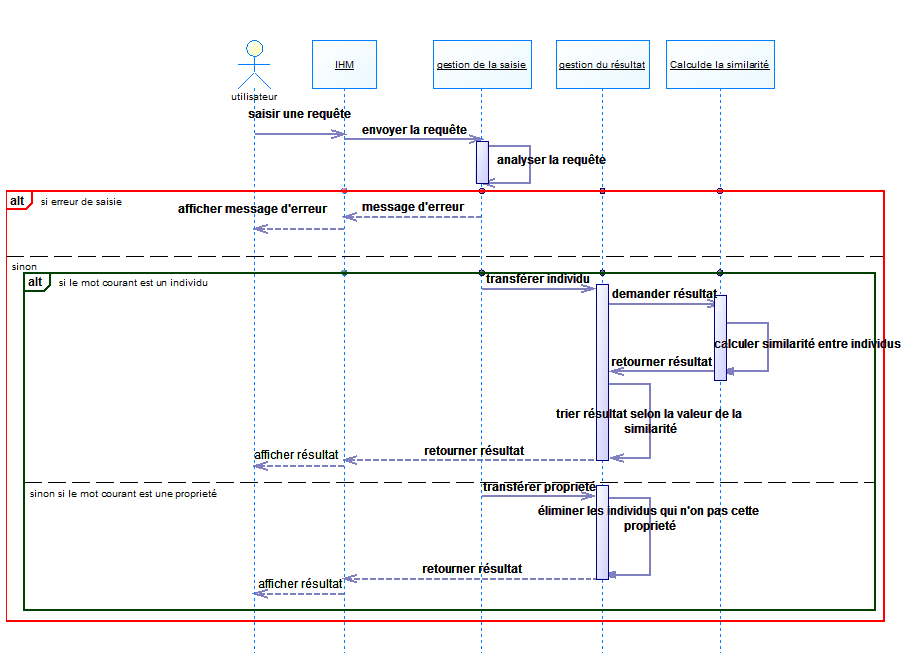
\includegraphics[width=17cm]{diag_sequence_detaille}\\
                    \caption{diagramme de sequences détaillé}\label{diagramme de sequence détaillé}
        \end{figure}
\section{Réalisation et tests}
    Aprés avoir analysé et défni les différentes parties qui constituent notre
    application, nous allons commencer la phase de réalisation et de tests. Celle-ci
    constitue le dernier volet de ce rapport. Elle a pour but d'exposer le travail
    achevé. Nous présenterons donc les différents Module réalisés et nous finissons par des tests.\\
    \subsection{Module de l'extraction des données}
                En se basent sur le diagramme des cas d'utilisation présenté précédemment, le traitement des requêtes ne peut se faire que lorsque le système a bien effecuté l'extraction des données à partir de l'ontologie en gardant les liens de parenté propres aux concepts et aux individus.\\
                Et pour garder ces caractéristiques nous avons  choisi de classer les entités de l'ontologie dans une structure de données arborescente.\\
                L'extraction des données se fait en parcourant le fichier qui décrit l'ontologie ,écrit en langage OWL et le système réagit à chaque ligne de code.\\
                Tout d'abord le système génère l'arborescence de l'ontologie en instanciant les classes ou les concepts et en établissant les liens de parenté entre eux au fur et à mesure du parcours du fichier.
                Ensuite il définit tous les individus de l'ontologie en ajoutant à chacun les  propriétés de types objet ou de type de donnée correspondantes.

    \subsection{Modéle MVC}
        Le modèle MVC est un modèle qui s'applique à la conception de tous les types d'applications qui présentent une interface homme-machine afin de séparer la couche métier de la couche IHM par l'intermédiaire du contrôleur. Chose qui facilite énormément la maintenance des logiciels\\
        Il découpe  l'application en trois couches distinctes:\\
        \begin{itemize}
            \item[\quad $\bullet$]
            Le contrôleur permet d’établir le lien entre la vue et le modèle. C’est le chef d’orchestre de l’application. Il ne fait qu’appeler des méthodes d'implémentation dans le  modèle ou dans la vue.
            \item[\quad $\bullet$]La vue représente l’interface homme-machine. Elle ne fait aucun traitement de données. Sa fonction se résume à la lecture de la requête de l’utilisateur et l’affichage du résultat.
            \item[\quad $\bullet$]C’est la couche métier de l’application : le modèle analyse la requête introduite par l’utilisateur, éffectue le traitement de cette requête en utilisant différents algorithmes performants de recherche selon la similarité.
        \end{itemize}
        \begin{figure}[H]
                    \centering
                    % Requires \usepackage{graphicx}
                    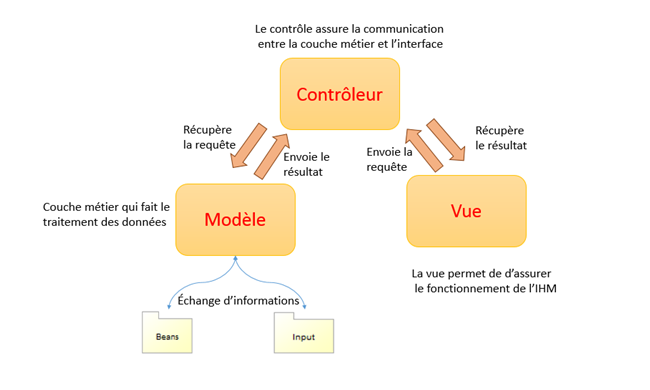
\includegraphics[width=17cm]{mvc}\\
                    \caption{Modéle MVC}\label{Modéle MVC}
        \end{figure}
    \subsection{Tests et validation}
        Tous nos tests dans cette partie seront basés sur un fichier écrit en langage OWL fourni dans l'annexe. La figure suivante générée par Protégé est une représentation graphique simplifiée de l'ontologie. Elle sert à suivre et à vérifier les tests que nous allons implémenter.\\
        \begin{figure}[H]
                    \centering
                    % Requires \usepackage{graphicx}
                    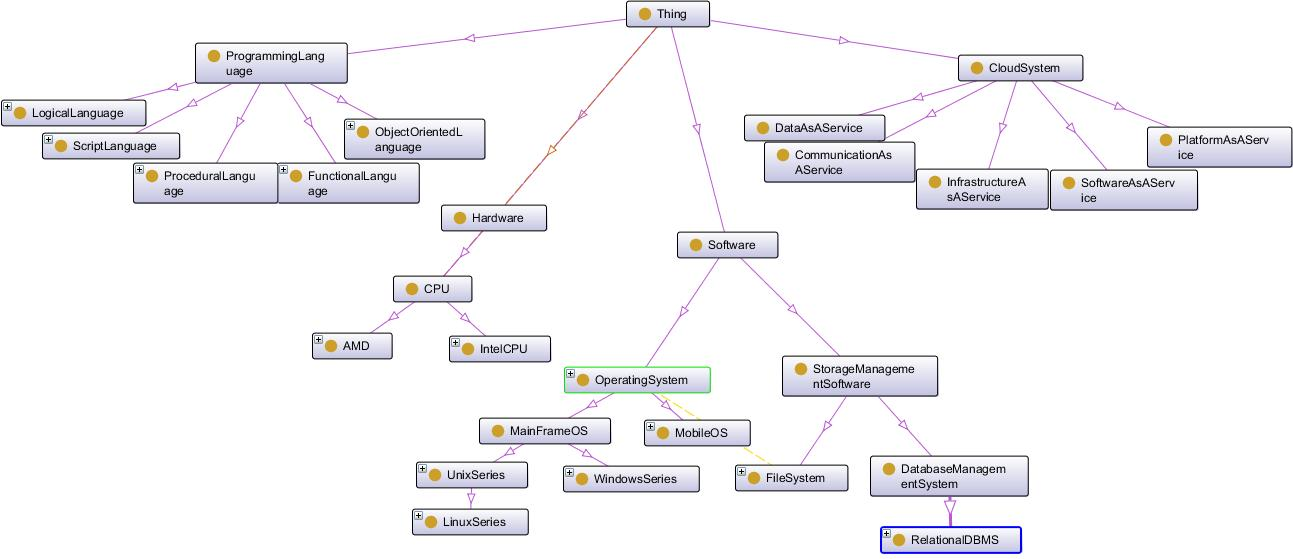
\includegraphics[width=15cm]{cloudle_ontologie}\\
                    \caption{Cloud ontologie}\label{cloud ontologie}
        \end{figure}

        \subsubsection{Extraction des données}
                        Pour tester l'extraction des données on indique quelle ontologie doit-on considérer. Dans notre cas nous avons choisi Cloud.owl. Il suffit d'appeler la méthode qui affiche l'ontologie tout en gardant les liens de parenté.\\
            \begin{figure}[H]
                    \centering
                    % Requires \usepackage{graphicx}
                    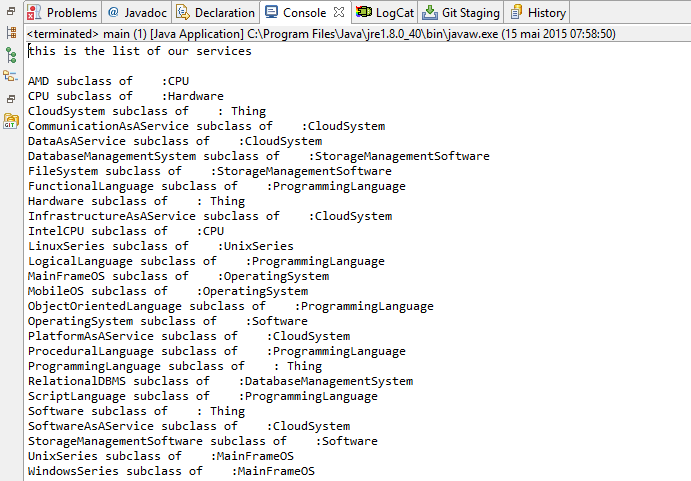
\includegraphics[width=14cm]{imprime_concepts}\\
                    \caption{impr1}\label{impr1}
        \end{figure}
        \subsubsection{Tests des requêtes}
            Lorsque l'utilisateur saisit une requête, deux cas de figure se présentent:\\
            \begin{itemize}
                \item[\quad $\bullet$]Si la requête n'est pas valide, un message d'erreur s'affiche sur l'écran en indiquant l'anomalie rencontrée à travers une boite de dialogue:
                    \begin{figure}[H]
                    \centering
                    % Requires \usepackage{graphicx}
                    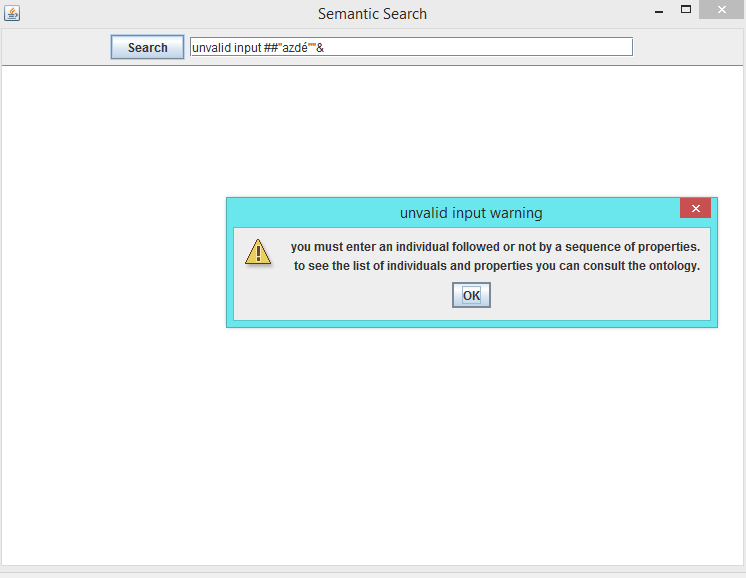
\includegraphics[width=14cm]{impr2}\\
                    \caption{impr2}\label{impr2}
                     \end{figure}
                \item[\quad $\bullet$]Si la requête est valide le résultat s'affiche sur l'écran:
                Soit les trois requêtes suivantes:
                    \begin{figure}[H]
                    \centering
                    % Requires \usepackage{graphicx}
                    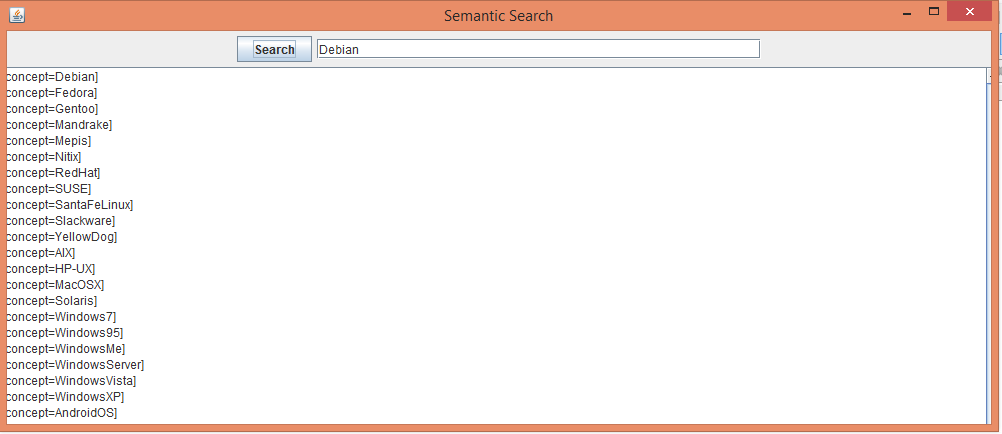
\includegraphics[width=15cm]{imr_debian}\\
                    \caption{imr debian}\label{imr debian}
                    \end{figure}
                     Lorsque l'utilisateur saisie le mot : Debian qui est un individu de l'ontologie de type système d'exploitation le système va afficher les individus classés par ordre de similarité décroissante.

                    \begin{figure}[H]
                    \centering
                    % Requires \usepackage{graphicx}
                    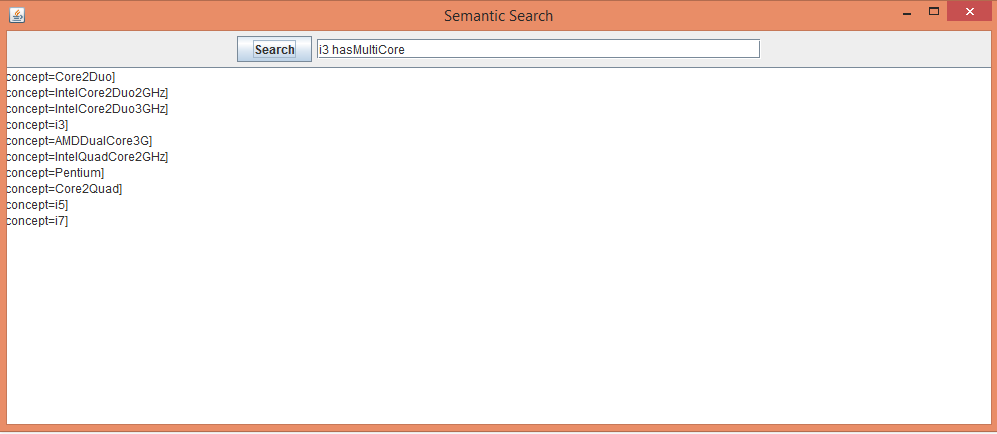
\includegraphics[width=15cm]{imprime_i3_hasMultiCore}\\
                    \caption{imprime i3 hasMultiCore}\label{imprime i3 hasMultiCore}
                    \end{figure}
                      Si l'utilisateur saisit la requête suivante: "i3 hasMultiCore" le système va afficher le résultat par ordre décroissant de la valeur de la similarité en éliminant les individus qui n'ont pas la propriété "hasMultiCore"
                    \begin{figure}[H]
                    \centering
                    % Requires \usepackage{graphicx}
                    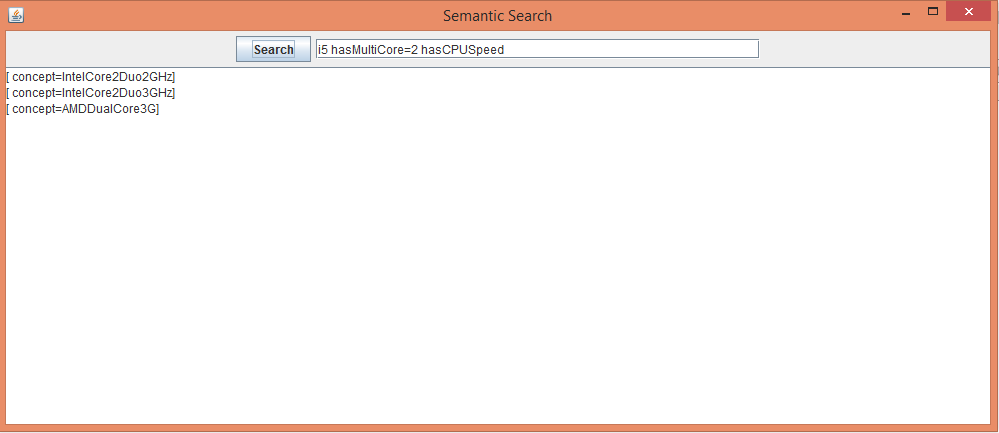
\includegraphics[width=15cm]{imprime_i5}\\
                    \caption{imprime i5 }\label{imprime i5}
                    \end{figure}
                    Lorsque l'utilisateur saisit : "i5 hasMultiCore=2 hasCPUSpeed" le système va chercher les individus similaires à i5 ,il va ensuite éliminer les entités qui n'ont pas la propriété hasMultiCore avec la valeur 2 et hasCPUSpeed et va trier le résultat par ordre décroissant de la similarité.

            \end{itemize}



\section{Conclusion}
    Dans ce chapitre nous avons introduit les outils utilisés pour l'implémentation de notre application. Suite à çela nous avons proposé la conception adéquate à ce système de recherche et nous avons terminé par la partie réalisation et tests.\\















